\documentclass[12pt,a4paper]{article}
\usepackage{calc}% http://ctan.org/pkg/calc
\usepackage[
  letterpaper,%
  textheight={47\baselineskip+\topskip},%
  textwidth={\paperwidth-126pt},%
  footskip=75pt,%
  marginparwidth=0pt,%
  top={\topskip+0.75in}]{geometry}% http://ctan.org/pkg/geometry
\usepackage{fancyhdr}% http://ctan.org/pkg/fancyhdr

\usepackage{graphicx}
%\usepackage{subcaption}

\usepackage{hyperref}
\usepackage{amsmath}
\usepackage{color}

\DeclareMathOperator{\Tr}{Tr}

\definecolor{orange}{rgb}{1,0.5,0}

\newcommand{\kpar}{k_{||}}
\newcommand{\kperp}{k_\perp}
\newcommand{\bvec}{\mathbf{b}}
\newcommand{\deriv}[2]{\frac{\partial #1}{\partial #2}}

\newcommand{\lr}[1]{\left( #1 \right)}
\newcommand{\slr}[1]{\left[ #1 \right]}

\newcommand{\ey}{\ensuremath{\mathbf{e}_y}}

\pagestyle{fancy}
%\fancyhead{}
\fancyfoot{}% Clear header & footer
%\fancyhead[L]{Electrostatic Ohm's law}% Set centered header
%\fancyhead[R]{ 22$^{nd}$ March 2014 }
\fancyfoot[C]{\thepage}% Set centered footer
\renewcommand{\headrulewidth}{0.5pt}% Add header rule

% Titling
\title{ Two-phase flow model }% Your title
\author{ Ben Dudson }% Your author
\date{ 23$^{rd}$ January 2018 }% Your date
\makeatletter
% Definition of proc.cls' \maketitle:
\def\@maketitle{% 
  \vbox to 1.25in{%
    \vskip 0.5em
    {\large \begin{tabular}[t]{ll}
        Title: & \@title \\
        Author: & \@author \\
        Date: & \@date \\
        Project: &
      \end{tabular}\par}
    \vfil}\noindent\hrulefill
    \vskip 2em}
\makeatother
\begin{document}
\maketitle % Produce title
\thispagestyle{fancy}% Override titling page style with fancy

\section{Model equations}

Equations for two or three immiscible incompressible fluids in 2D is
solved using the vorticity formulation. The fluid velocity
$\mathbf{u}$ is calculated using $\mathbf{u} =
\nabla\times\mathbf{\psi}$, where in 2D only only one component of the
stream function $\psi$ is needed. All code, inputs and analysis
scripts used here are available at
\url{https://github.com/bendudson/two-phase-flow}.

\subsection{Fluid interface tracking}

A Volume of Fluid (VOF) approach is used to track the interface
between the two phases. A colour field $c$ is $0$ in one fluid, and
$1$ in the other, transitioning between $0$ and $1$ at the boundary
between them. The density $\rho$ and kinematic viscosity $\nu$ are
given by
\begin{eqnarray}
\rho &=& \left(1-c\right)\rho_0 + c \rho_1 \\
\nu &=& \left(1-c\right)\nu_0 + c \nu_1 \\
\end{eqnarray}
The colour moves with the flow velocity $\mathbf{u}$:
\begin{equation}
\frac{\partial c}{\partial t} + \mathbf{u}\cdot\nabla c = 0
\end{equation}

This advection equation is solved using the following algorithm:
\begin{enumerate}
\item The stream function $\psi$ is interpolated onto cell corners, then derivatives taken along cell edges to calculate the flow
velocity through the cell faces.
\item A $1^{st}$-order upwinding algorithm is used to advect
  the field $c$ through cell faces.
\item In order to control the diffusion which would smear out
  the sharp boundary over time, a regularised anti-diffusion
  term is added, which acts to steepen the boundary between the
  fluids\footnote{K.K.So, X.Y.Hu, N.A.Adams J.Comp.Phys. 230 (2011) 5155-5177}. 
\end{enumerate}

\subsection{Momentum and vorticity}

Starting from the momentum equation:

\begin{equation}
\frac{\partial}{\partial t}\left(\rho \mathbf{u}\right) + \mathbf{u}\cdot\nabla\left(\rho\mathbf{u}\right) = -\nabla p - g\mathbf{e}_x + \rho\nu\nabla^2\mathbf{u} - \mathbf{F}_s
\end{equation}
take the $y$ component of the curl of this equation, to get
the vorticity in 2D ($x-z$).

The surface tension force per unit area of surface is
\begin{equation}
\mathbf{F}_A = \sigma\kappa\left(c\right)\mathbf{n}
\end{equation}
where $\sigma$ is a scalar coefficient of surface tension,
in Newtons per meter; $\kappa$ is the surface curvature (units 1/m); $\mathbf{n}$ is the unit vector normal to the surface.
This is represented using the Continuum Surface Force (CSF) formulation\footnote{J.U.Brackbill, D.B.Kothe, C.Zemach J.Comp.Phys 100, 335-354 (1992)} as a force per unit volume, given by:
\begin{equation}
\mathbf{F}_s = \sigma\kappa\left(c\right)\nabla c
\end{equation}
When integrated over a surface, $\nabla c$ gives $\left[c\right]$, which transitions from 0 to 1 across a surface, so recovers the force per unit area given above. 
The curvature $\kappa$ is related to the surface normal
\begin{equation}
\kappa = \nabla\cdot\left(\mathbf{n}\right)
\end{equation}
The surface normal can be approximated using the $c$ field:
\begin{equation}
\mathbf{n} = \nabla c / \left|\nabla c\right|
\end{equation}

Taking the curl of the surface force, the surface force term can be written 
as a Poisson bracket:
\begin{eqnarray}
\mathbf{e}_y\cdot\nabla\times \mathbf{F}_s &=& \mathbf{e}_y\cdot\nabla\left(\sigma\kappa\right)\times\nabla c \\
&=& -\mathbf{e}_y\times\nabla\left(\sigma\kappa\right)\cdot\nabla c \\
&=& -\left[\sigma\kappa, c\right]
\end{eqnarray}

Finally this gives the equation for the vorticity $\omega$:
\begin{equation}
\frac{\partial\omega}{\partial t} = -\left[\psi, \omega\right] - g\frac{\partial\rho}{\partial z} + \nabla\cdot\left(\nu\nabla \omega\right) - \left[\sigma\kappa, c\right]
\end{equation}

In this model the Poisson brackets are implemented using Arakawa's $2^{nd}$-order advection scheme.

\subsection{Viscosity}

The kinematic viscosity $\nu$ is calculated using the weighted VOF as described above. The viscosity of each fluid is set by the input options \texttt{viscosity0}, \texttt{viscosity1} and \texttt{viscosity2}. These can be constants:
\begin{verbatim}
viscosity0 = 1e-6
\end{verbatim}
or can depend on time:
\begin{verbatim}
viscosity0 = 1e-6 + 1e-6 * t
\end{verbatim}
where \texttt{t} has the same units as the output (i.e. seconds if using SI units everywhere).

The viscosity can also depend on the local velocity shear $\gamma$ (units $s^-1$), which is represented by \texttt{y}. For example a shear-thinning non-newtonian fluid might be modelled as\footnote{G.P.Roberts, H.A.Barnes, P.Carew 2001 \url{https://www.sciencedirect.com/science/article/pii/S0009250901002913}}:
\begin{verbatim}
viscosity0 = 1e-4 / (1 + (y/1e-4)^2)
\end{verbatim}
which is
\[
\nu = \frac{10^{-4}}{1 + \left(\gamma/10^{-4}\right)^2}
\]
The calculation of $\gamma$ is given in section~\ref{sec:shear_rate}.

Three models for the viscosity term are included, chosen in the input file
by setting \texttt{visc\_method}.

\subsubsection{Simple vorticity diffusion}
\label{sec:visc0}

The simplest model assumes constant density and viscosity
\begin{equation}
  \frac{\partial\omega}{\partial t} = \nu\nabla^2\omega + \cdots
  \label{eq:vorticity_visc}
\end{equation}
This is a diffusion equation for the vorticity.

{\bf Note:} Only use this if density and viscosity are constant.
If either of these is not true then using this expression results in
unphysical solutions (unstable oscillations).

\subsubsection{Corrected vorticity diffusion (default)}

If $\mu$ is not constant, then the simple viscosity term can become an
energy source rather than a sink. To see this, calculate the change
in kinetic energy by multiplying the vorticity equation~\ref{eq:vorticity_visc}
by $\psi$ and integrating over the simulation volume.

\begin{eqnarray}
  \psi \frac{\partial\omega}{\partial t} &=& \psi\nu\nabla^2\omega \\
  \frac{\partial\psi\omega}{\partial t} - \frac{\partial\psi}{\partial t}\omega &=& \nabla\cdot\left(\psi\nu\nabla\omega\right) - \nabla\omega\cdot\nabla\left(\psi\nu\right) \\
  &=&  \nabla\cdot\left(\psi\nu\nabla\omega\right) -\nu \nabla\omega\cdot\nabla\psi - \psi\nabla\omega\cdot\nabla\nu 
\end{eqnarray}
The right hand side becomes:
\begin{eqnarray}
  \nabla\omega\cdot\nabla\psi &=& \nabla\cdot\lr{\omega\nabla\psi} - \omega\nabla^2\psi \\
  &=& \nabla\cdot\lr{\omega\nabla\psi} - \rho\left|\nabla^2\psi\right|^2
\end{eqnarray}
where the last step assumes $\rho$ is constant. The left hand side
\begin{eqnarray}
  \psi\omega = \psi\nabla\cdot\lr{\rho\nabla\psi} &=& \nabla\cdot\lr{\rho\psi\nabla\psi} -\rho\nabla\psi\cdot\nabla\psi  \\
  &=& \nabla\cdot\lr{\rho\psi\nabla\psi} -\rho\left|\nabla\psi\right|^2 \\
  \frac{\partial\psi}{\partial t}\omega = \frac{\partial\psi}{\partial t}\nabla\cdot\lr{\rho\nabla\psi} &=& \nabla\cdot\lr{\rho\frac{\partial\psi}{\partial t}\nabla\psi} - \rho\nabla\psi\cdot\nabla\frac{\partial\psi}{\partial t} \\
  &=& \nabla\cdot\lr{\rho\frac{\partial\psi}{\partial t}\nabla\psi} - \frac{1}{2}\rho\frac{\partial}{\partial t}\left|\nabla\psi\right|^2
\end{eqnarray}
After integrating over the domain, the divergence terms turn into surface integrals over the boundary. If $\psi = 0$ or $\nabla\psi\cdot d\mathbf{S}$ perpendicular to the surface $d\mathbf{S}$ then these surface terms vanish. Therefore:
\begin{eqnarray}
 -\frac{\partial}{\partial t}\left[\frac{1}{2}\rho\left|\nabla\psi\right|^2\right] &=& \rho\left|\nabla^2\psi\right|^2 - \psi\nabla\omega\cdot\nabla\nu
\end{eqnarray}
{\bf NOTE}: Parts of this derivation assume $\rho$ is constant.
    
The left hand side represents the change in kinetic energy; the first term on the right
is a damping term which depends on the gradient of the flow speed.
Note that it always has the same sign (damping). The last term can be positive
or negative, depending on the gradients of vorticity
$\omega$ and viscosity $\nu$. This term can be cancelled by adding a term
to the vorticity equation:

\begin{equation}
  \frac{\partial\omega}{\partial t} = \nu\nabla^2\omega + \nabla\omega\cdot\nabla\nu = \nabla\cdot\left(\nu \nabla\omega\right)
  \label{eq:vorticity_visc1}
\end{equation}

\subsubsection{Stress tensor derivation}

In the momentum equation the stress tensor $\Pi$ appears as
\begin{equation}
\frac{\partial}{\partial t}\left(\rho \mathbf{u}\right) = \ldots + \nabla\cdot\Pi 
\end{equation}
and for a Newtonian fluid can be written as
\begin{equation}
  \Pi_{ij} = \mu\slr{\deriv{u_i}{x_j} + \deriv{u_j}{u_i} - \frac{2}{3}\delta_{ij} \deriv{u_k}{x_k}}
\end{equation}
where $\mu = \rho\nu$ depends on fluid density and kinematic viscosity $\nu$.
For an incompressible fluid the last term vanishes ($\nabla\cdot\mathbf{u} = 0$).

The vorticity equation viscosity term is found by applying
$\ey\cdot\nabla\times$ to the momentum equation. In tensor notation
this is
\begin{eqnarray}
  \Pi_\omega &=& \epsilon_{ykj}\partial_k\slr{\partial_i\lr{\mu \partial_j u_i
                                            + \mu \partial_i u_j}} \\
  &=& \lr{\partial_z^2 - \partial_x^2}\lr{\mu\partial_x u_z + \mu \partial_z u_x} + \partial_{xz}^2\lr{2\mu\partial_x u_x - 2\mu \partial_zu_z}
\end{eqnarray}

The components of the velocity can be calculated from the definition:
\begin{equation}
  \mathbf{u} = \nabla\times\lr{\ey \psi} = \nabla\psi \times\ey
\end{equation}
so
\begin{equation}
  u_i = \epsilon_{ijy}\partial_j \psi \qquad u_x = -\partial_z\psi \qquad u_z = \partial_x\psi
\end{equation}
so
\[
\partial_x u_x - \partial_z u_z = -2\partial_{xz}^2\psi
\]
\[
\partial_x u_z + \partial_zu_x = \partial_x^2\psi - \partial_z^2\psi
\]
Inserting and simplifying gives
\begin{eqnarray}
  \Pi_\omega &=& -\mu\lr{\partial_x^2 + \partial_z^2}^2\psi - \lr{\partial_x \mu - \partial_z\mu}\lr{\partial_x \psi - \partial_z \psi} - 4\lr{\partial_{xz}^2\mu}\lr{\partial_{xz}^2\psi} \\
  &=& -\nabla_\perp^2\lr{\mu \nabla_\perp^2\psi} + 2\slr{\partial_x^2\mu \partial_z^2\psi + \partial_z^2\mu \partial_x^2\psi - 2\lr{\partial_{xz}^2\mu}\lr{\partial_{xz}^2\psi}}
\end{eqnarray}
where $\nabla_\perp^2 = \partial_x^2 + \partial_z^2$

The Poisson bracket can be written as
\begin{equation}
\left[f, g\right] = \partial_zf\partial_xg - \partial_xf\partial_zg
\end{equation}
so
\begin{equation}
  \Pi_\omega = -\nabla_\perp^2\lr{\mu \nabla_\perp^2\psi} - 2\slr{\partial_x\mu,\partial_z\psi} - 2\slr{\partial_x\psi, \partial_z\mu}
\end{equation}

In the case that $\mu$ is constant, this reduces to the simple model (section~\ref{sec:visc0}).

\subsection{Calculation of curvature}
\label{sec:curvature}

Two methods for calculating the curvature $\kappa$ are implemented: A finite difference method and the Height Function method. 

The finite difference (FD) method uses a smoothed function of $c$, and calculates $\kappa = \nabla\cdot\mathbf{n}$ using finite differences\footnote{}.

The Height Function (HF) method is a $2^{nd}$-order scheme which integrates the function $c$ and then takes finite differences of those integrals\footnote{M.Sussman J.Comp.Phys. 187 (2003) 110-136}.
\section{Tests}

\subsection{Stationary bubble}

A standard test of two-phase fluid models is to test the
magnitude of parasitic (non-physical) flows around a stationary bubble. These arise from the calculation of curvature in VOF type schemes.
\begin{figure}[h]
\centering
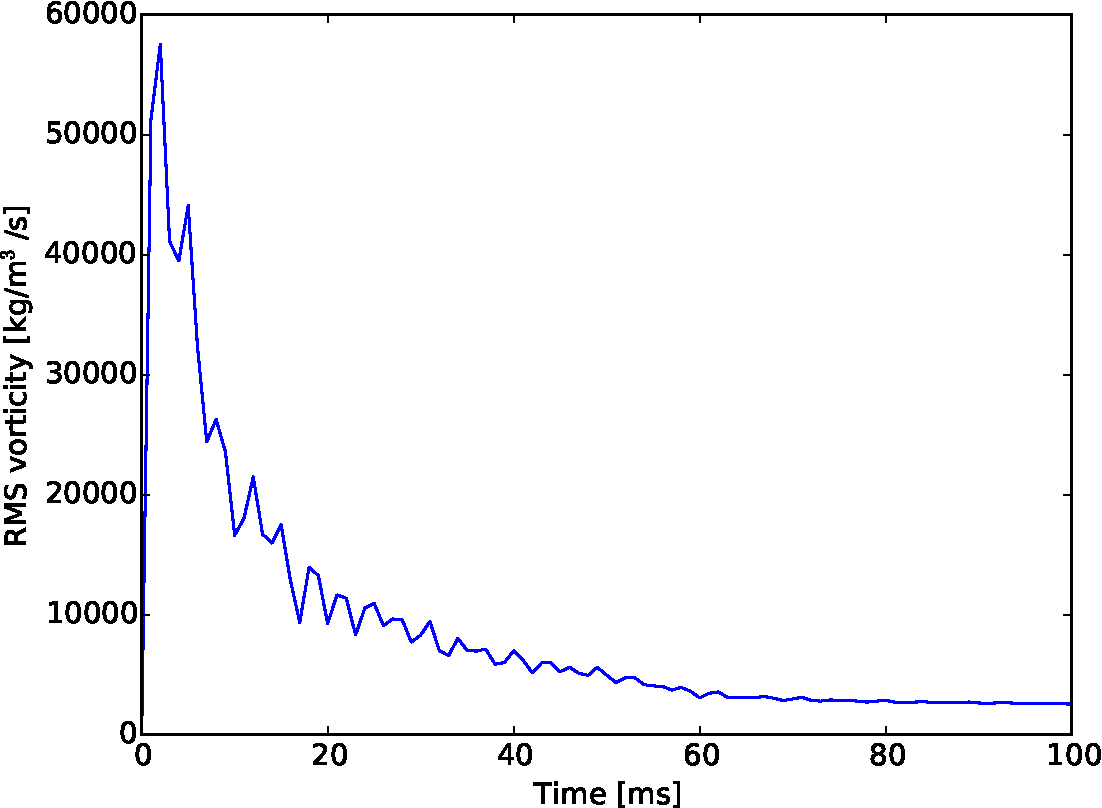
\includegraphics[width=0.45\textwidth]{bubble_vorticity.pdf}
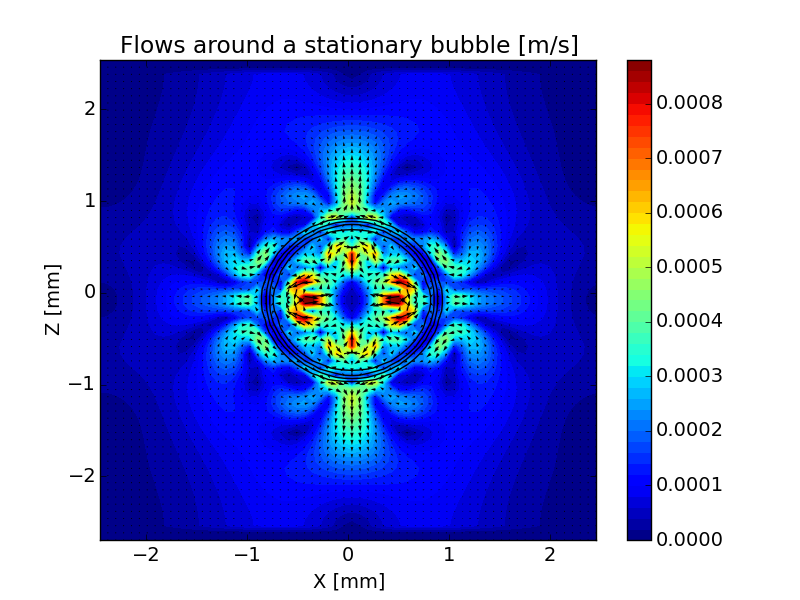
\includegraphics[width=0.45\textwidth]{bubble_flows.png}
\caption{Simulation of a stationary bubble of radius $\sim 1$mm. {\bf Left}: Evolution of the average (Root-Mean-Square) vorticity in the domain as a function of time. {\bf Right}: Final state showing flow magnitude (colours), direction (arrows), and the boundary of the bubble (black contours).}
\label{fig:bubble}
\end{figure}
Figure~\ref{fig:bubble} shows the evolution and final state of
a circular bubble. The two fluids have the same density $\rho=1000$kg/m$^3$ and kinematic viscosity $\nu=10^{-6}$m$^2$/s (approximately water). The surface tension is $\sigma=72$mN/m, similar to that for water-air interfaces. The curvature is calculated using the Finite Difference method. 

The vorticity initially increases and the width of the interface region grows. After around $60$ms a steady state is reached, with parasitic flows of the order of $1$mm/s.

\subsection{Capillary wave dispersion}

A sinusoidal perturbation of an interface between two fluids is simulated, based on simulations in [Denner 2017]\footnote{F.Denner et al. Computers and Fluids 143 (2017) 59-72}. Both fluids have the same density $\rho=1$kg/m$^3$ and kinematic viscosity $\nu = 1.6394\times 10^{−3}$m$^2$/s. The surface tension between the two fluids is $\sigma=0.25\pi^{-3}$N/m. The domain is $\lambda$ in width ($z$ direction here), and $3\lambda$ in height ($x$ direction). Results for wavelengths $\lambda=1$m and $\lambda=0.1$m are shown in figure~\ref{fig:capillary}.
\begin{figure}[h]
\centering
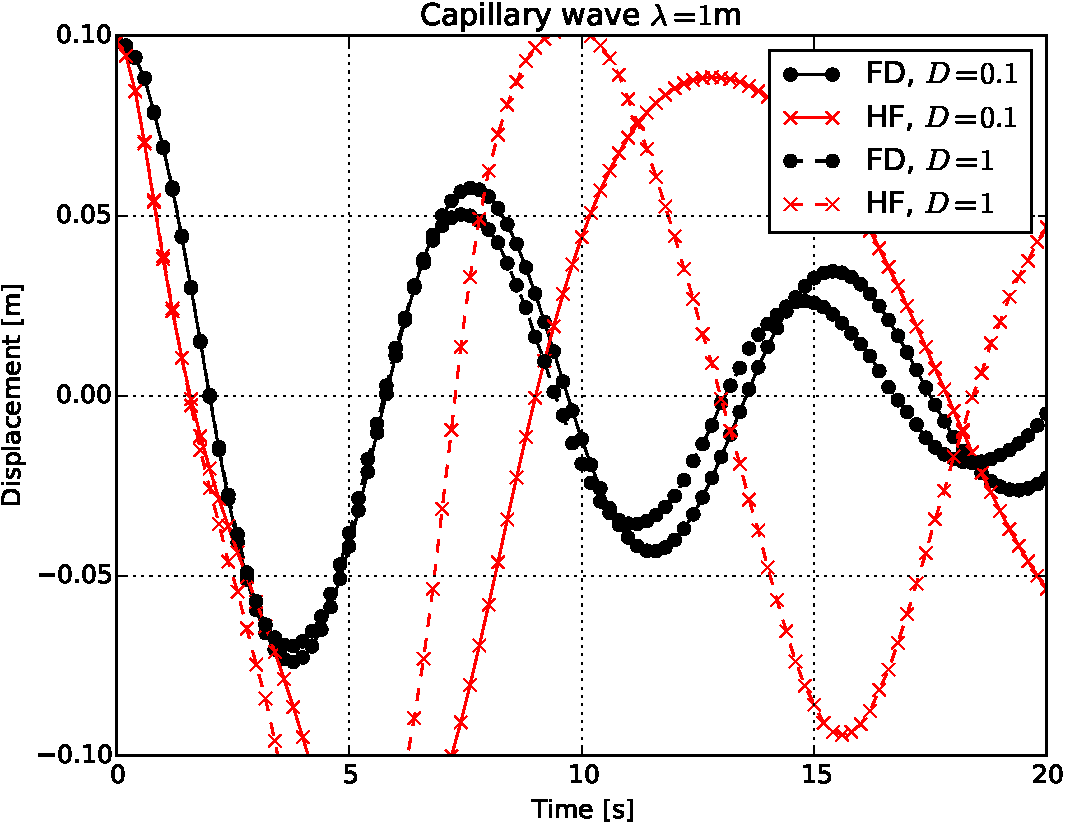
\includegraphics[width=0.45\textwidth]{capillary_2.pdf}
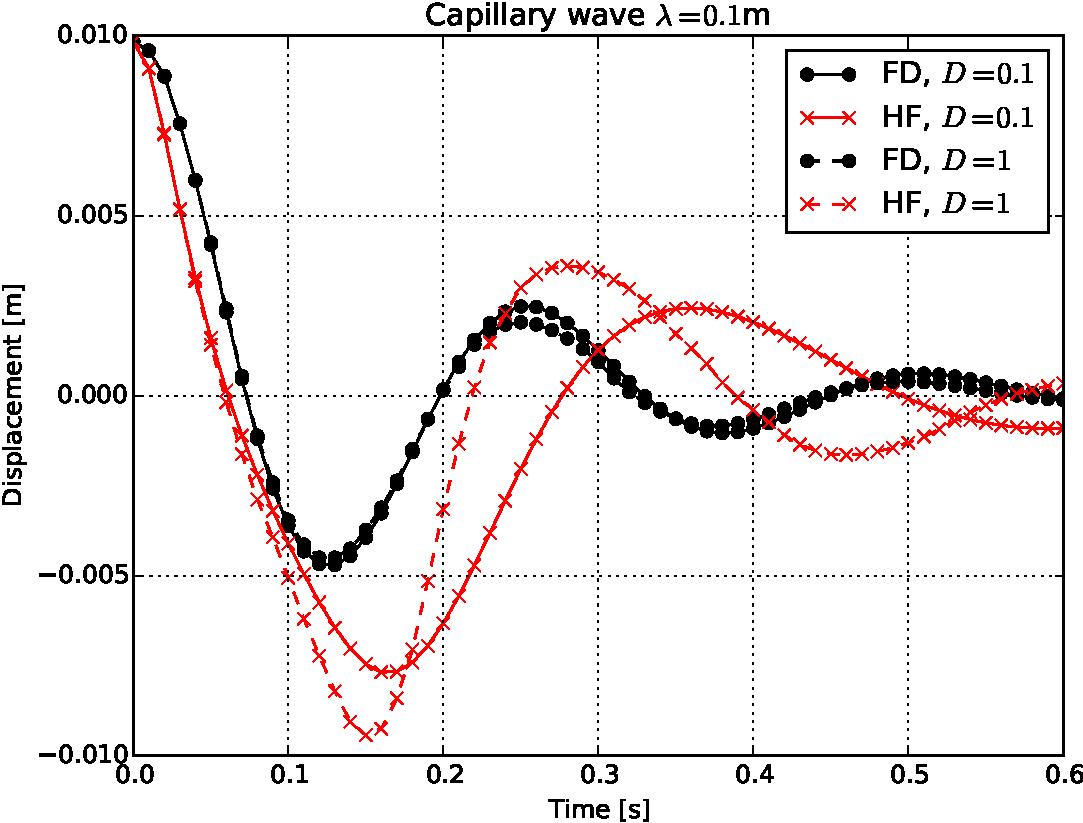
\includegraphics[width=0.45\textwidth]{capillary_1.pdf}
\caption{Evolution of the amplitude of a standing capillary wave, for comparison with figure 2 of [Denner 2017]}
\label{fig:capillary}
\end{figure}
This indicates that whilst the Finite Difference calculation of curvature gives good agreement, the Height Function method does not. Sharpening the interface by increasing the anti-diffusion $D$ improves the result.

\section{Calculation of shear rate}
\label{sec:shear_rate}

The expression for the shear $\gamma$ was derived from the discussion here\footnote{DOI: \texttt{10.1615/AtoZ.n.non-newtonian\_fluids} \url{http://www.thermopedia.com/content/986/}}:
\begin{equation}
\gamma^2 = \frac{1}{2}\left[\Tr{\left(\mathbf{e}^2\right)} - \left(\Tr\left(\mathbf{e}\right)\right)^2\right]
\end{equation}
where $\mathbf{e}$ is the strain rate tensor:
\begin{eqnarray}
  \mathbf{e} &=& \nabla\mathbf{u} + \left(\nabla\mathbf{u}\right)^T \\
  &=& \left(\begin{array}{cc}
    2\frac{\partial u_x}{\partial x} & \frac{\partial u_x}{\partial z} + \frac{\partial u_z}{\partial x} \\
    \frac{\partial u_x}{\partial z} + \frac{\partial u_z}{\partial x} & 2\frac{\partial u_x}{\partial z} \end{array}\right) \label{eq:strain_rate} \\
  &=&  \left(\begin{array}{cc}
  e_{xx} & e_{xz} \\
  e_{xz} & e_{zz} \end{array}\right)
\end{eqnarray}

From this we can get
\[
\mathbf{e}^2 =  \left(\begin{array}{cc}
  e_{xx}^2 + e_{xz}^2 &  \\
   & e_{zz}^2 + e_{xz}^2 \end{array}\right)
\]
(where the off-diagonal terms are not needed, so not given).
Hence
\begin{eqnarray*}
  \Tr\left(\mathbf{e}^2\right) &=& e_{xx}^2 + 2e_{xz}^2 + e_{zz}^2 \\
  \Tr\left(\mathbf{e}\right) &=& e_{xx} + e_{zz} \\
  \left(\Tr\left(\mathbf{e}\right)\right)^2 &=& e_{xx}^2 + 2e_{xx}e_{zz} + e_{zz}^2
\end{eqnarray*}
And so
\begin{equation}
  \gamma^2 = \frac{1}{2}\left(2e_{xz}^2 - e_{xx}e_{zz}\right)
\end{equation}

Inserting the expressions from equation~\ref{eq:strain_rate} gives:
\[
2e_{xz}^2 - e_{xx}e_{zz} = 4\left(\frac{\partial u_x}{\partial z} + \frac{\partial u_z}{\partial x}\right)^2 - 4\frac{\partial u_x}{\partial x}\frac{\partial u_z}{\partial z}
\]
Then using $\mathbf{u} = \nabla\times\left(\psi\hat{\mathbf{y}}\right)$ gives
\[
u_x = -\frac{\partial \psi}{\partial z} \qquad u_z = \frac{\partial \psi}{\partial x}
\]
so
\[
\gamma^2 = 2\left(\frac{\partial^2 \psi}{\partial x^2} - \frac{\partial^2 \psi}{\partial z^2}\right)^2 + 2\left(\frac{\partial^2 \psi}{\partial x\partial z}\right)^2
\]

\end{document}
